%|====================| config
\documentclass[12pt, A4]{article}
\usepackage[margin=1.8cm]{geometry}
\usepackage[T1]{fontenc} 
\usepackage[utf8]{inputenc}
\usepackage[spanish, es-noshorthands]{babel} 

%|====================| packages
\usepackage{amsmath}
\usepackage{amssymb}
\usepackage{booktabs}
\usepackage{graphicx}
\graphicspath{{images/}}
\usepackage{hyperref}
\usepackage{algorithm}
\usepackage{algpseudocode}
\usepackage{subcaption}
\usepackage{fancyhdr}

%|====================| customization
\pagestyle{fancy}
\fancyhead[R]{UTEC 2025-1}
\fancyhead[L]{Computación Paralela y Distribuida}
\renewcommand\contentsname{ÍNDICE}
\title{\textbf{Computación Paralela y Distribuida}}


%|====================| doc
\begin{document}

% Declaración del nuevo bloque para algoritmos
\algblock{ParFor}{EndParFor}
\algnewcommand\algorithmicparfor{\textbf{for}}
\algnewcommand\algorithmicpardo{\textbf{pardo}}
\algnewcommand\algorithmicendparfor{\textbf{end for}}
\algrenewtext{ParFor}[1]{\algorithmicparfor\ #1\ \algorithmicpardo}
\algrenewtext{EndParFor}{\algorithmicendparfor}

\include{title.tex}
\tableofcontents
\newpage

\section{Introducción}

El algoritmo de \textbf{Marching Squares} se distingue por su naturaleza intrínsecamente paralelizable, una característica que emana de su proceso no iterativo y su operación directa sobre una estructura de grilla. Este proyecto se adentra en un análisis exhaustivo y una comparación detallada de los tiempos de cómputo, empleando el algoritmo en su forma \textbf{iterativa y sin precisión adaptativa}. Esta particular elección metodológica es crucial, ya que nos permite observar el peor caso de ejecución, donde la complejidad temporal del algoritmo se manifiesta en su forma cuadrática.

Para comprender su funcionamiento, es esencial entender que el algoritmo opera iterando sobre una superficie bidimensional, examinando cada una de sus subdivisiones. Este proceso permite la generación de líneas de contorno a partir de un campo escalar, un método fundamental en gráficos por computadora y procesamiento de imágenes.

Para la realización de las pruebas de rendimiento, hemos utilizado el clúster \textbf{Khipu}. Adicionalmente, se desarrolló e implementó un renderizador específico para \textbf{visualizar} los resultados de cada ejecución, asegurando así la coherencia y validez de los datos obtenidos. Paralelamente, se integró una implementación en \textbf{CUDA}; si bien las pruebas con esta versión se realizaron con una única GPU, se consideró una variedad de modelos de GPU para expandir la perspectiva de la experimentación.

Finalmente, se abordará un análisis de \textbf{escalabilidad fuerte y débil}, centrándose exclusivamente en las implementaciones para CPU con la arquitectura x86. Para ello, se presentarán gráficos y otros datos relevantes que ilustrarán de manera clara el rendimiento y la eficiencia alcanzados.
    
\newpage
\section{Algoritmo}
El algoritmo de \textbf{Marching Squares} opera sobre una grilla bidimensional de tamaño $N \times N$ para identificar y trazar contornos (también conocidos como isolíneas o isotérmicas) a partir de un campo escalar. La lógica fundamental del algoritmo procesa cada celda de la grilla de manera independiente, como se detalla en el siguiente pseudocódigo:

\begin{algorithm}
\caption{Marching Squares}
\begin{algorithmic}[1]
\State Sea R un conjunto el conjunto de resultados.
\For{$i = 0$ to $N - 1$}
    \For{$j = 0$ to $N - 1$}
        \State Obtener valores del campo escalar en los vértices A, B, C, D de la celda $(i,j)$
        \State Calcular el caso como número binario según los signos de A, B, C, D
        \State Interpolar cruces con el isovalor en los bordes, si hay cambio de signo
        \State Según el \textbf{caso}, generar uno o dos segmentos de línea dentro de la celda
        \State Añadir los segmentos al conjunto de resultados
    \EndFor
\EndFor
\State \Return R 
\end{algorithmic}
\end{algorithm}

El caso utilizado depende de cómo se codifica en un entero de 4 bits, permitiendo un máximo de 16 posibilidades que se resuelven con un simple switch.

\subsection{Paradigma de Paralelización}

Para la implementación paralela del algoritmo se selecciona el paradigma de \textbf{Paralelismo de Datos}, adecuado debido a la independencia inherente del procesamiento de cada celda. El cálculo para una celda $(i, j)$ no depende de las celdas adyacentes, permitiendo división en subproblemas autónomos ejecutables concurrentemente.

\subsection{Modelo PRAM}

%El modelo PRAM (Parallel Random Access Machine) desarrollado para Marching Squares conceptualiza la ejecución paralela del algoritmo. %Este modelo asume que múltiples procesadores pueden acceder a una memoria global compartida de manera simultánea.
%
%\textbf{:}
%\begin{itemize}
%    \item \textbf{INPUT:}
%    \begin{itemize}
%        \item $f(x, y)$: Función del campo escalar bidimensional.
%        \item \texttt{grid\_size}: Dimensión de la grilla $N \times N$.
%        \item \texttt{min\_v}, \texttt{max\_v}: Rango de valores en el campo escalar (o el rango de la grilla espacial).
%    \end{itemize}
%    \item \textbf{OUTPUT:}
%    \begin{itemize}
%        \item $R$: Un conjunto de segmentos de línea, donde $R = \{((x_1, y_1), (x_2, y_2)) \in \mathbb{R}^2 \times \mathbb{R}^2 \mid %f(x_1, y_1) = f(x_2, y_2) = c, \text{ con } c \in [\text{min\_v}, \text{max\_v}] \}$.
%    \end{itemize}
%\end{itemize}
%
\begin{algorithm}[H]
\footnotesize % o \scriptsize
\caption{Marching Squares - PRAM}
\begin{algorithmic}[1]
\Statex \textbf{Input:} $f(x, y)$, \texttt{grid\_size}, \texttt{min\_v}, \texttt{max\_v}
\Statex \textbf{Output:} Conjunto de líneas $R$
\State $DT \gets (\texttt{max\_v} - \texttt{min\_v}) / \texttt{grid\_size}$
\State Declarar \texttt{line\_buffer[1..grid\_size]} como arreglo de conjuntos
\ParFor{$i = 1$ to $\texttt{grid\_size}$ } \Comment{Inicializar iteraciones}
    \State \texttt{line\_buffer[i]} $\gets \emptyset$    
    \For{$j = 1$ to $\texttt{grid\_size}$}
        \State Calcular $(x1, y1), (x2, y2)$ coordenadas de la celda
        \State Evaluar $A = f(x1, y1), B = f(x2, y1), C = f(x2, y2), D = f(x1, y2)$
        \State $case \gets (D > 0) \ll 3 \,|\, (C > 0) \ll 2 \,|\, (B > 0) \ll 1 \,|\, (A > 0)$
        \State $d_{bottom} = \texttt{interpolate}(A, B) \cdot DT$
        \State $d_{right} = \texttt{interpolate}(B, C) \cdot DT$
        \State $d_{top} = \texttt{interpolate}(C, D) \cdot DT$
        \State $d_{left} = \texttt{interpolate}(D, A) \cdot DT$
        
        \State Añadir a \texttt{line\_buffer}[i] los lineas de acuerdo a $case$.     
    \EndFor
\EndParFor
\State $R \gets \emptyset$ \Comment{Realizar reducción global}
\For{$i = 1$ to \texttt{grid\_size}}
    \State $R \gets R \cup \texttt{line\_buffer[i]}$
\EndFor
\State \Return $R$
\end{algorithmic}
\end{algorithm}

El modelo PRAM asume acceso \textbf{CREW (Concurrent Read, Exclusive Write)} donde múltiples procesadores leen simultáneamente los datos de entrada, pero escriben en buffers locales para evitar contención. La fase final de reducción combina los resultados locales.

\subsection{Complejidad y Speedup Teórico}

La complejidad secuencial es $T_s = O(n^2)$ para procesar $n \times n$ celdas. En paralelo con $p$ procesadores:
\[
T_p = \frac{n^2}{p} + p
\]
donde el segundo término representa overhead de paralelización. El speedup teórico resulta:
\[
S(p) = \frac{n^2}{\frac{n^2}{p} + p}
\]
Este modelo predice que el speedup crece con $p$ pero se limita por el overhead, coherente con la Ley de Amdahl.



\subsection{Implementación C++}
Las implementaciones utilizan aritmética de doble precisión (\texttt{double}) para x86 y punto flotante simple (\texttt{float}) para CUDA. Los experimentos se ejecutaron en el cluster Khipu con SLURM.

\subsubsection{Iteración I}
Implementación secuencial base que establece la línea de referencia. Utiliza bucles anidados para recorrer la grilla $n \times n$ con complejidad $O(n^2)$. Almacena resultados directamente en \texttt{std::deque<LineSegment>} sin optimizaciones de paralelización.

\subsubsection{Iteración II}
Paralelización básica con OpenMP utilizando scheduling estático por filas. Implementa buffers locales por thread y agregación mediante secciones críticas. La escalabilidad está limitada por la contención en la fusión final de resultados.

\subsubsection{Iteración III}
Optimización avanzada que introduce \textit{move semantics} y indexación directa por thread ID. Reduce significativamente la contención mediante fusión post-paralela y pre-asignación de memoria. Alcanza eficiencias de hasta 85\% en configuraciones multinúcleo.

\subsubsection{Iteración IV}
Implementación CUDA que representa un cambio paradigmático hacia paralelismo masivo en GPU. Utiliza un thread por celda de grilla con configuración de bloques 16×16. Incluye 8 funciones matemáticas especializadas y manejo exhaustivo de errores CUDA.

    
\section{Resultados}
\subsection{Gráficas Speedup}

A continuación se presentan las gráficas de speedup para distintos tamaños de grilla, donde se evalúa el rendimiento en función del número de procesadores. Cada experimento fue realizado manteniendo el tamaño de problema fijo, representando un análisis de escalabilidad fuerte.

\begin{figure}[H]
    \centering

    \begin{subfigure}{0.48\textwidth}
        \centering
        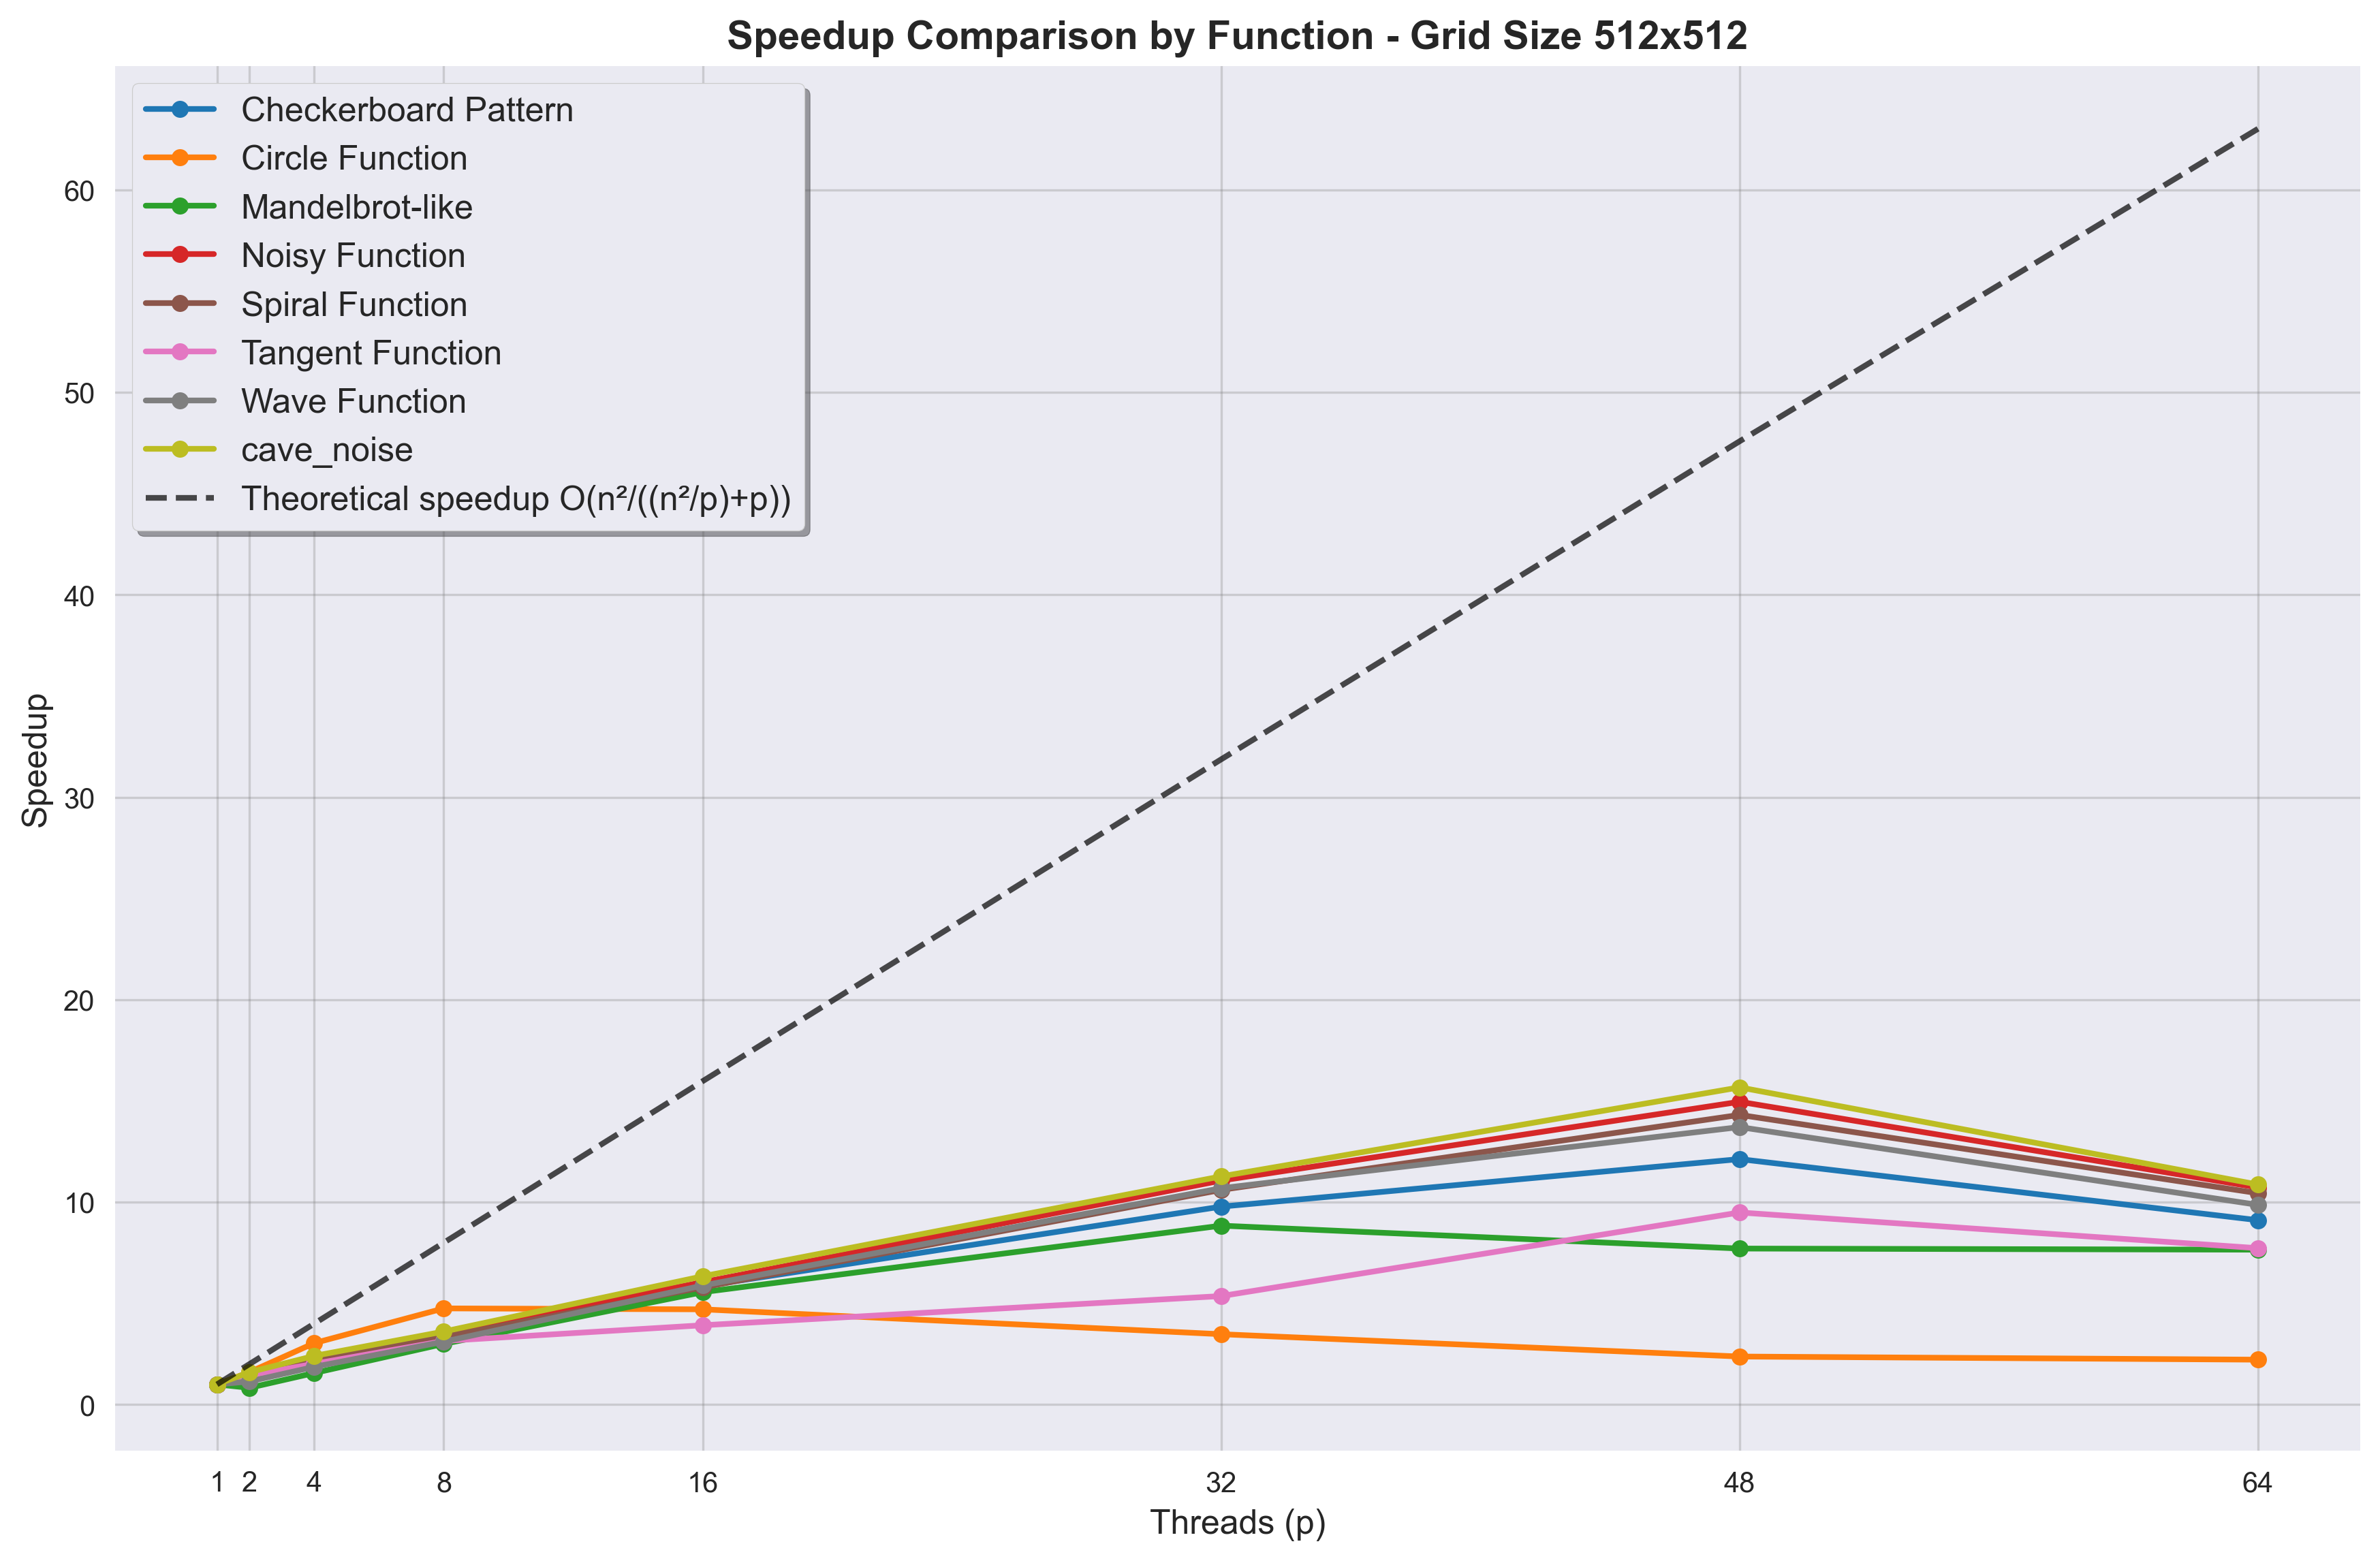
\includegraphics[height=5cm]{images/speedup_comparison_grid_512.png}
        \caption{Grilla 512}
        \label{fig:speedup_512}
    \end{subfigure}\hspace*{\fill}
    \begin{subfigure}{0.48\textwidth}
        \centering
        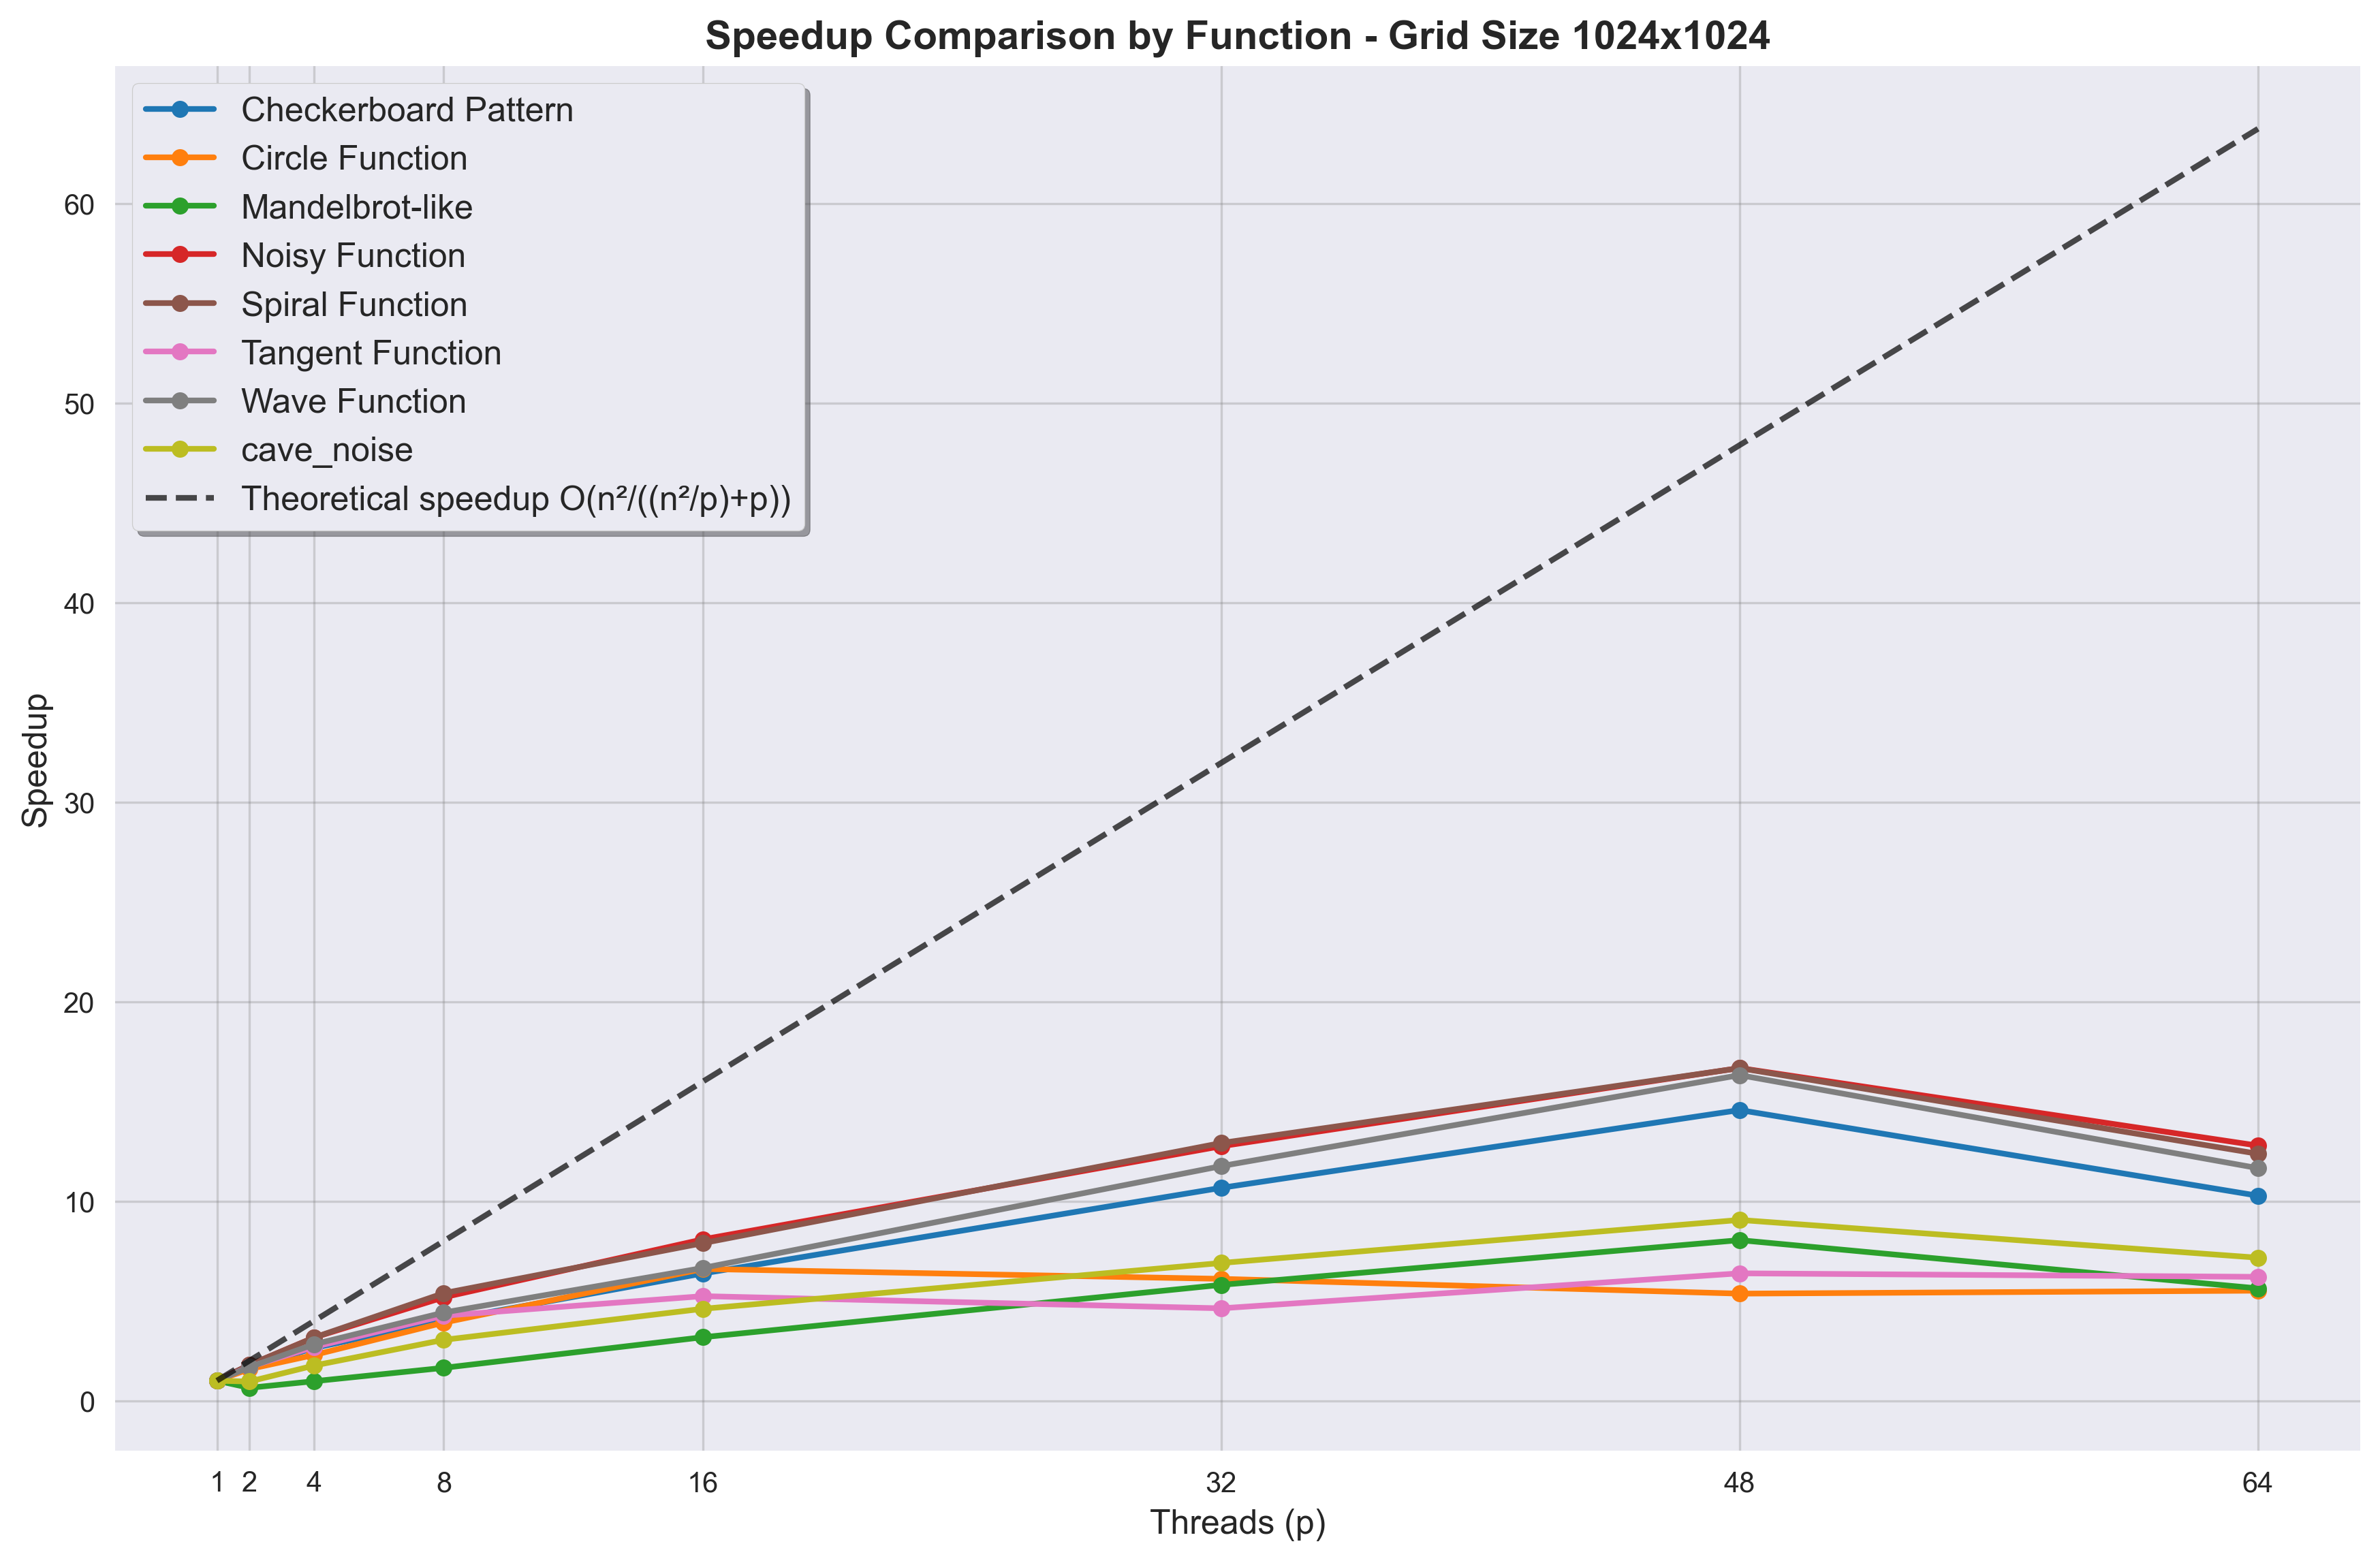
\includegraphics[height=5cm]{images/speedup_comparison_grid_1024.png}
        \caption{Grilla 1024}
        \label{fig:speedup_1024}
    \end{subfigure}

    \medskip

    \begin{subfigure}{0.48\textwidth}
        \centering
        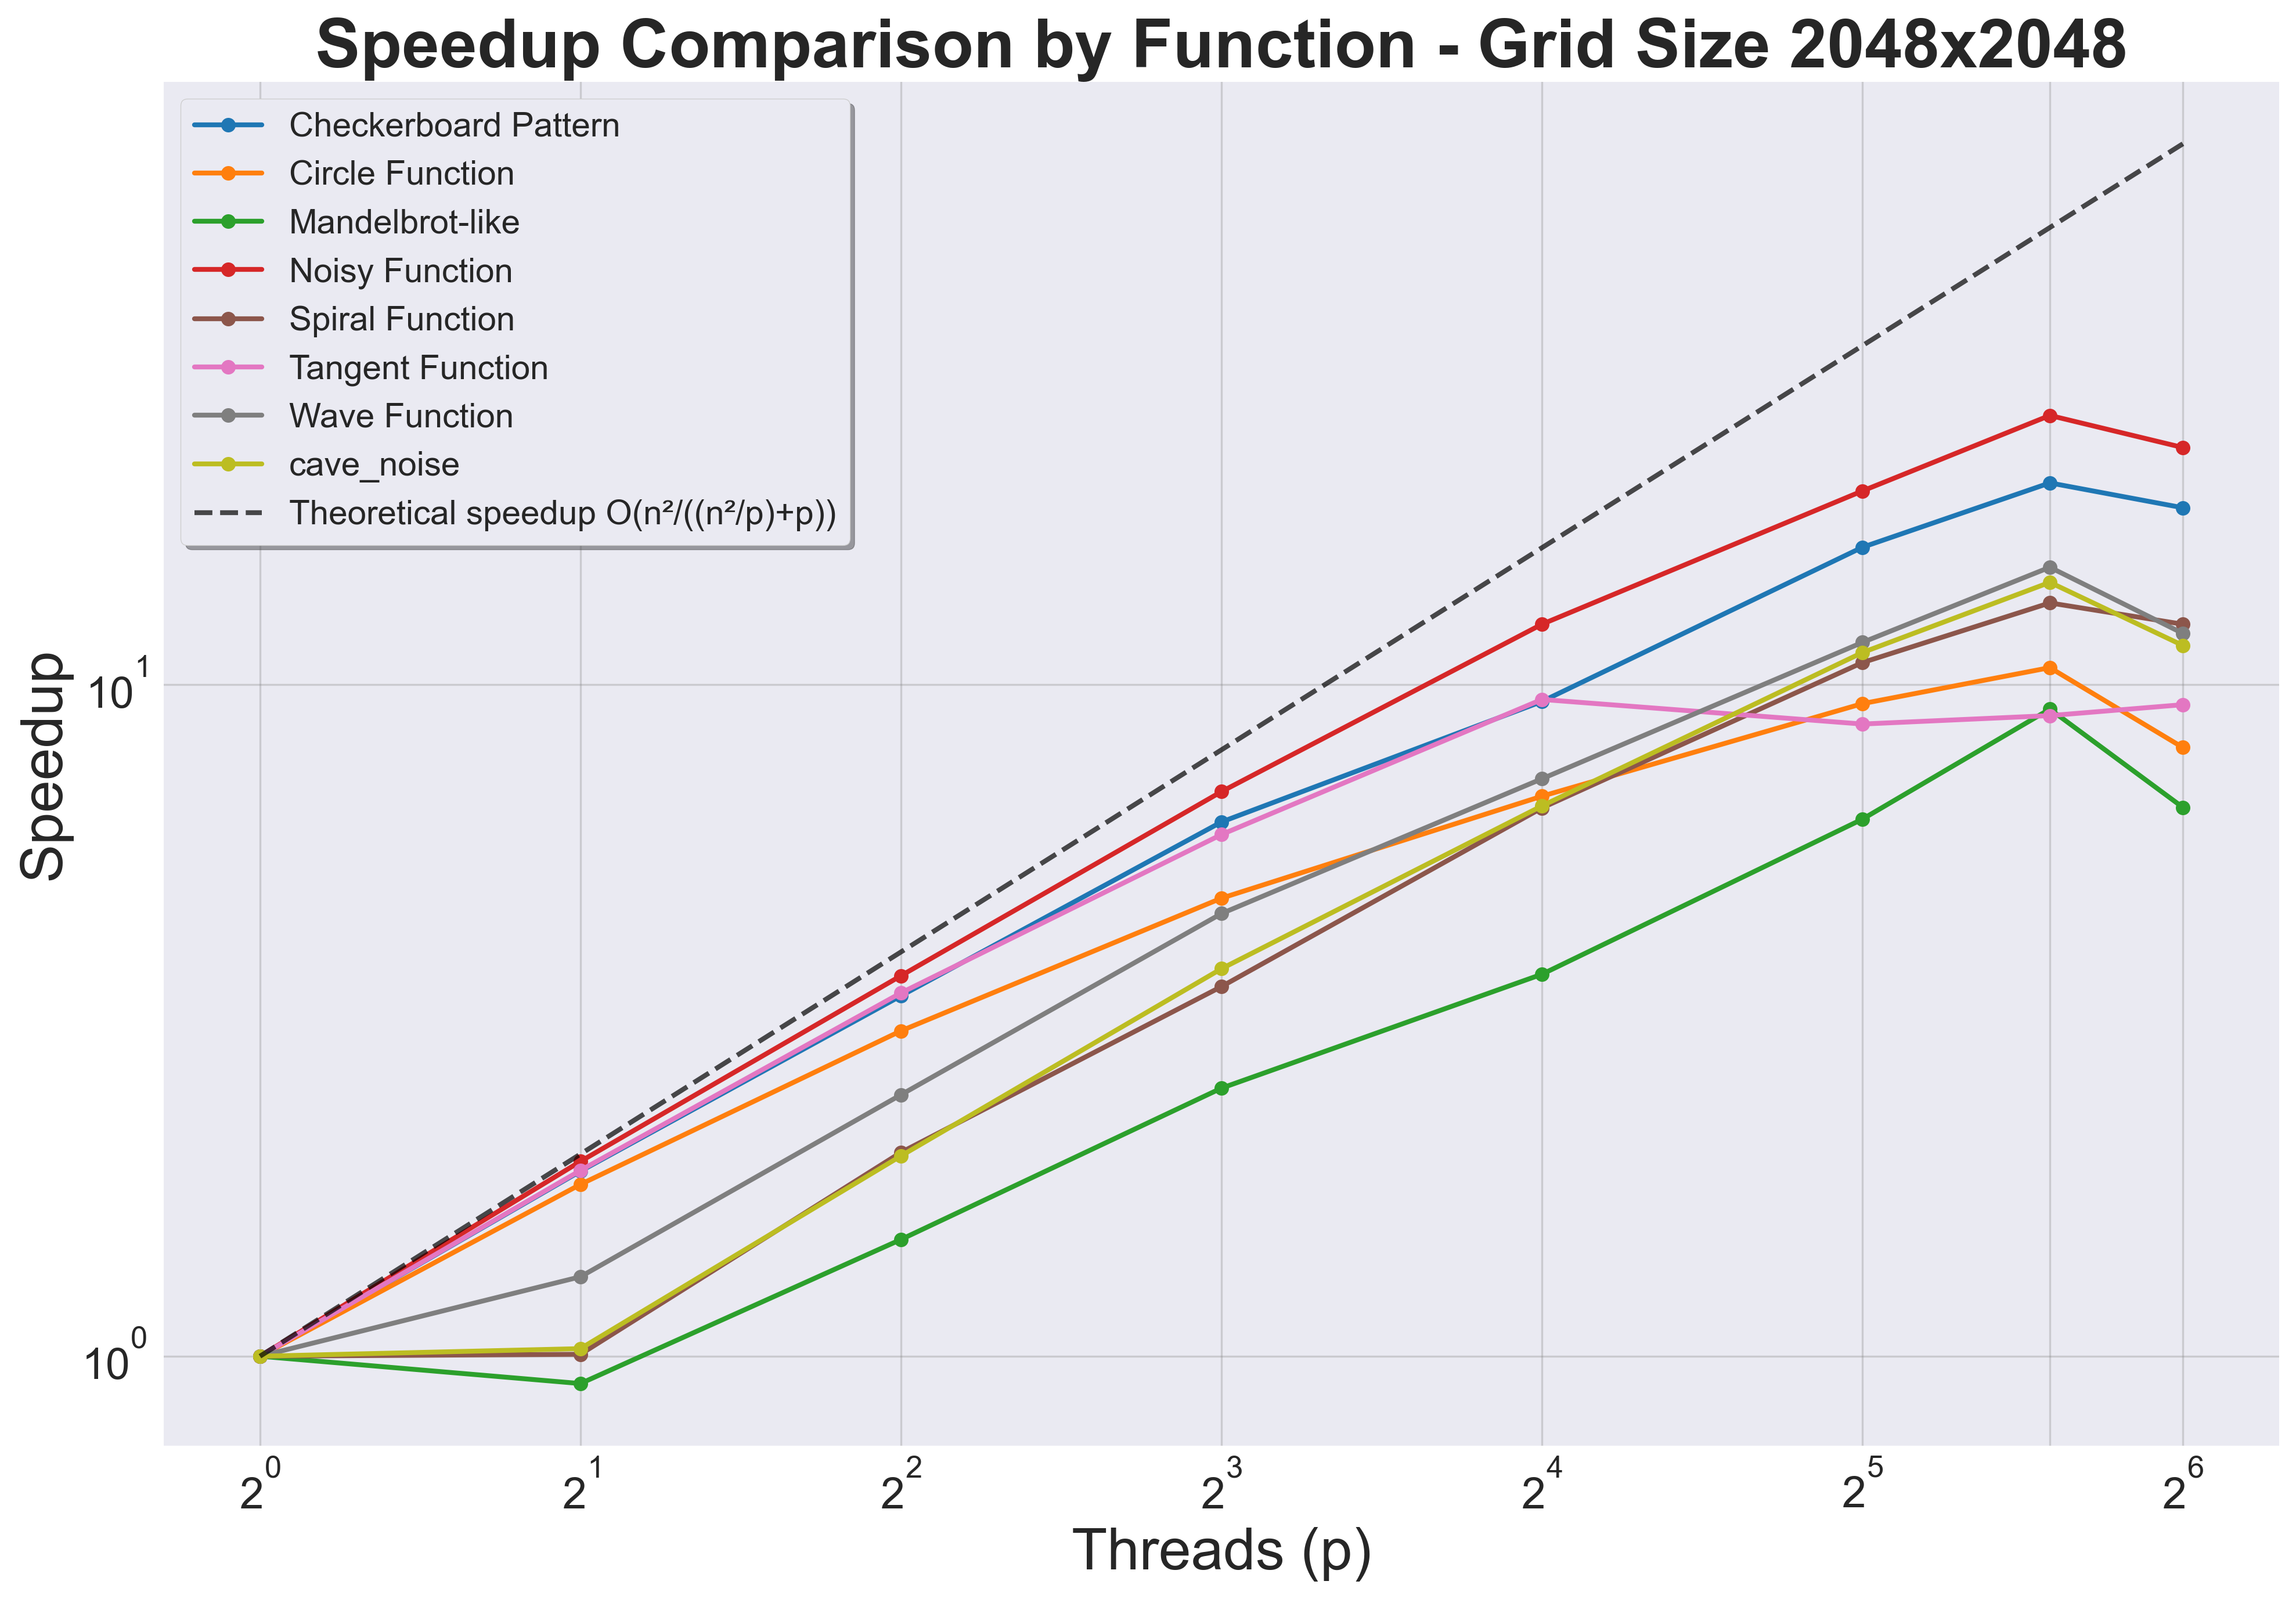
\includegraphics[height=5cm]{images/speedup_comparison_grid_2048.png}
        \caption{Grilla 2048}
        \label{fig:speedup_2048}
    \end{subfigure}\hspace*{\fill}
    \begin{subfigure}{0.48\textwidth}
        \centering
        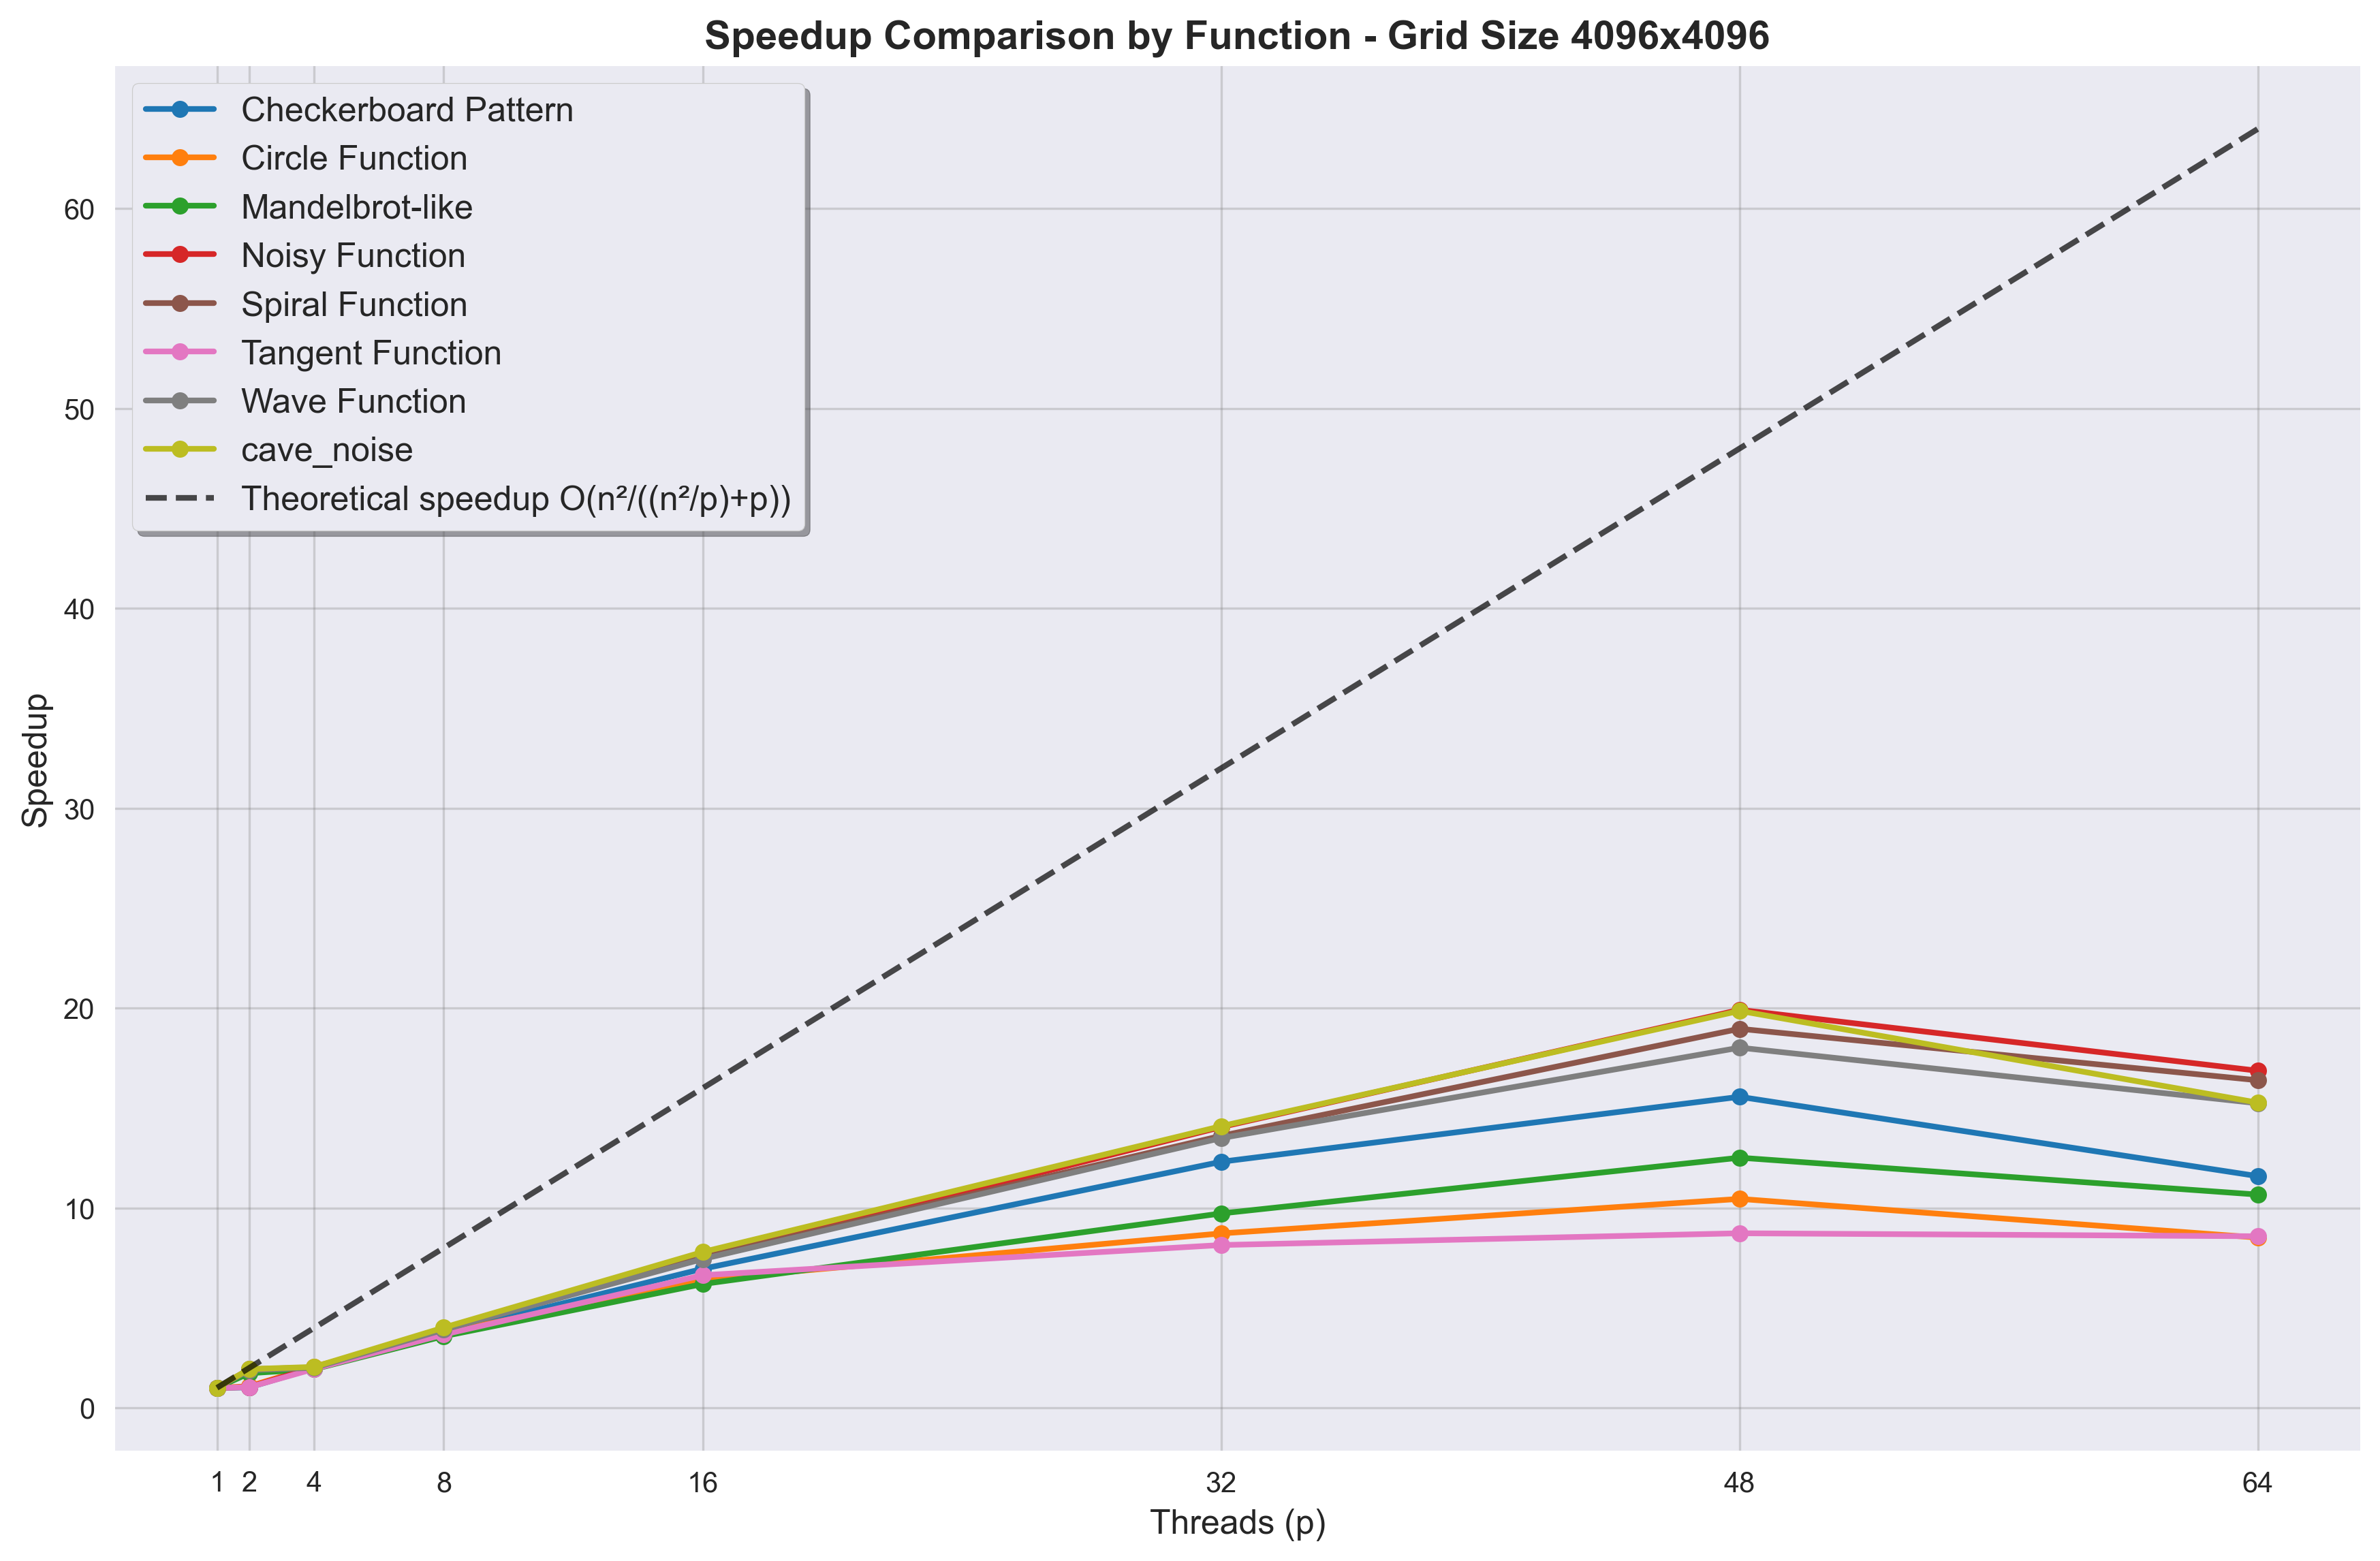
\includegraphics[height=5cm]{images/speedup_comparison_grid_4096.png}
        \caption{Grilla 4096}
        \label{fig:speedup_4096}
    \end{subfigure}

    \medskip

    \begin{subfigure}{0.48\textwidth}
        \centering
        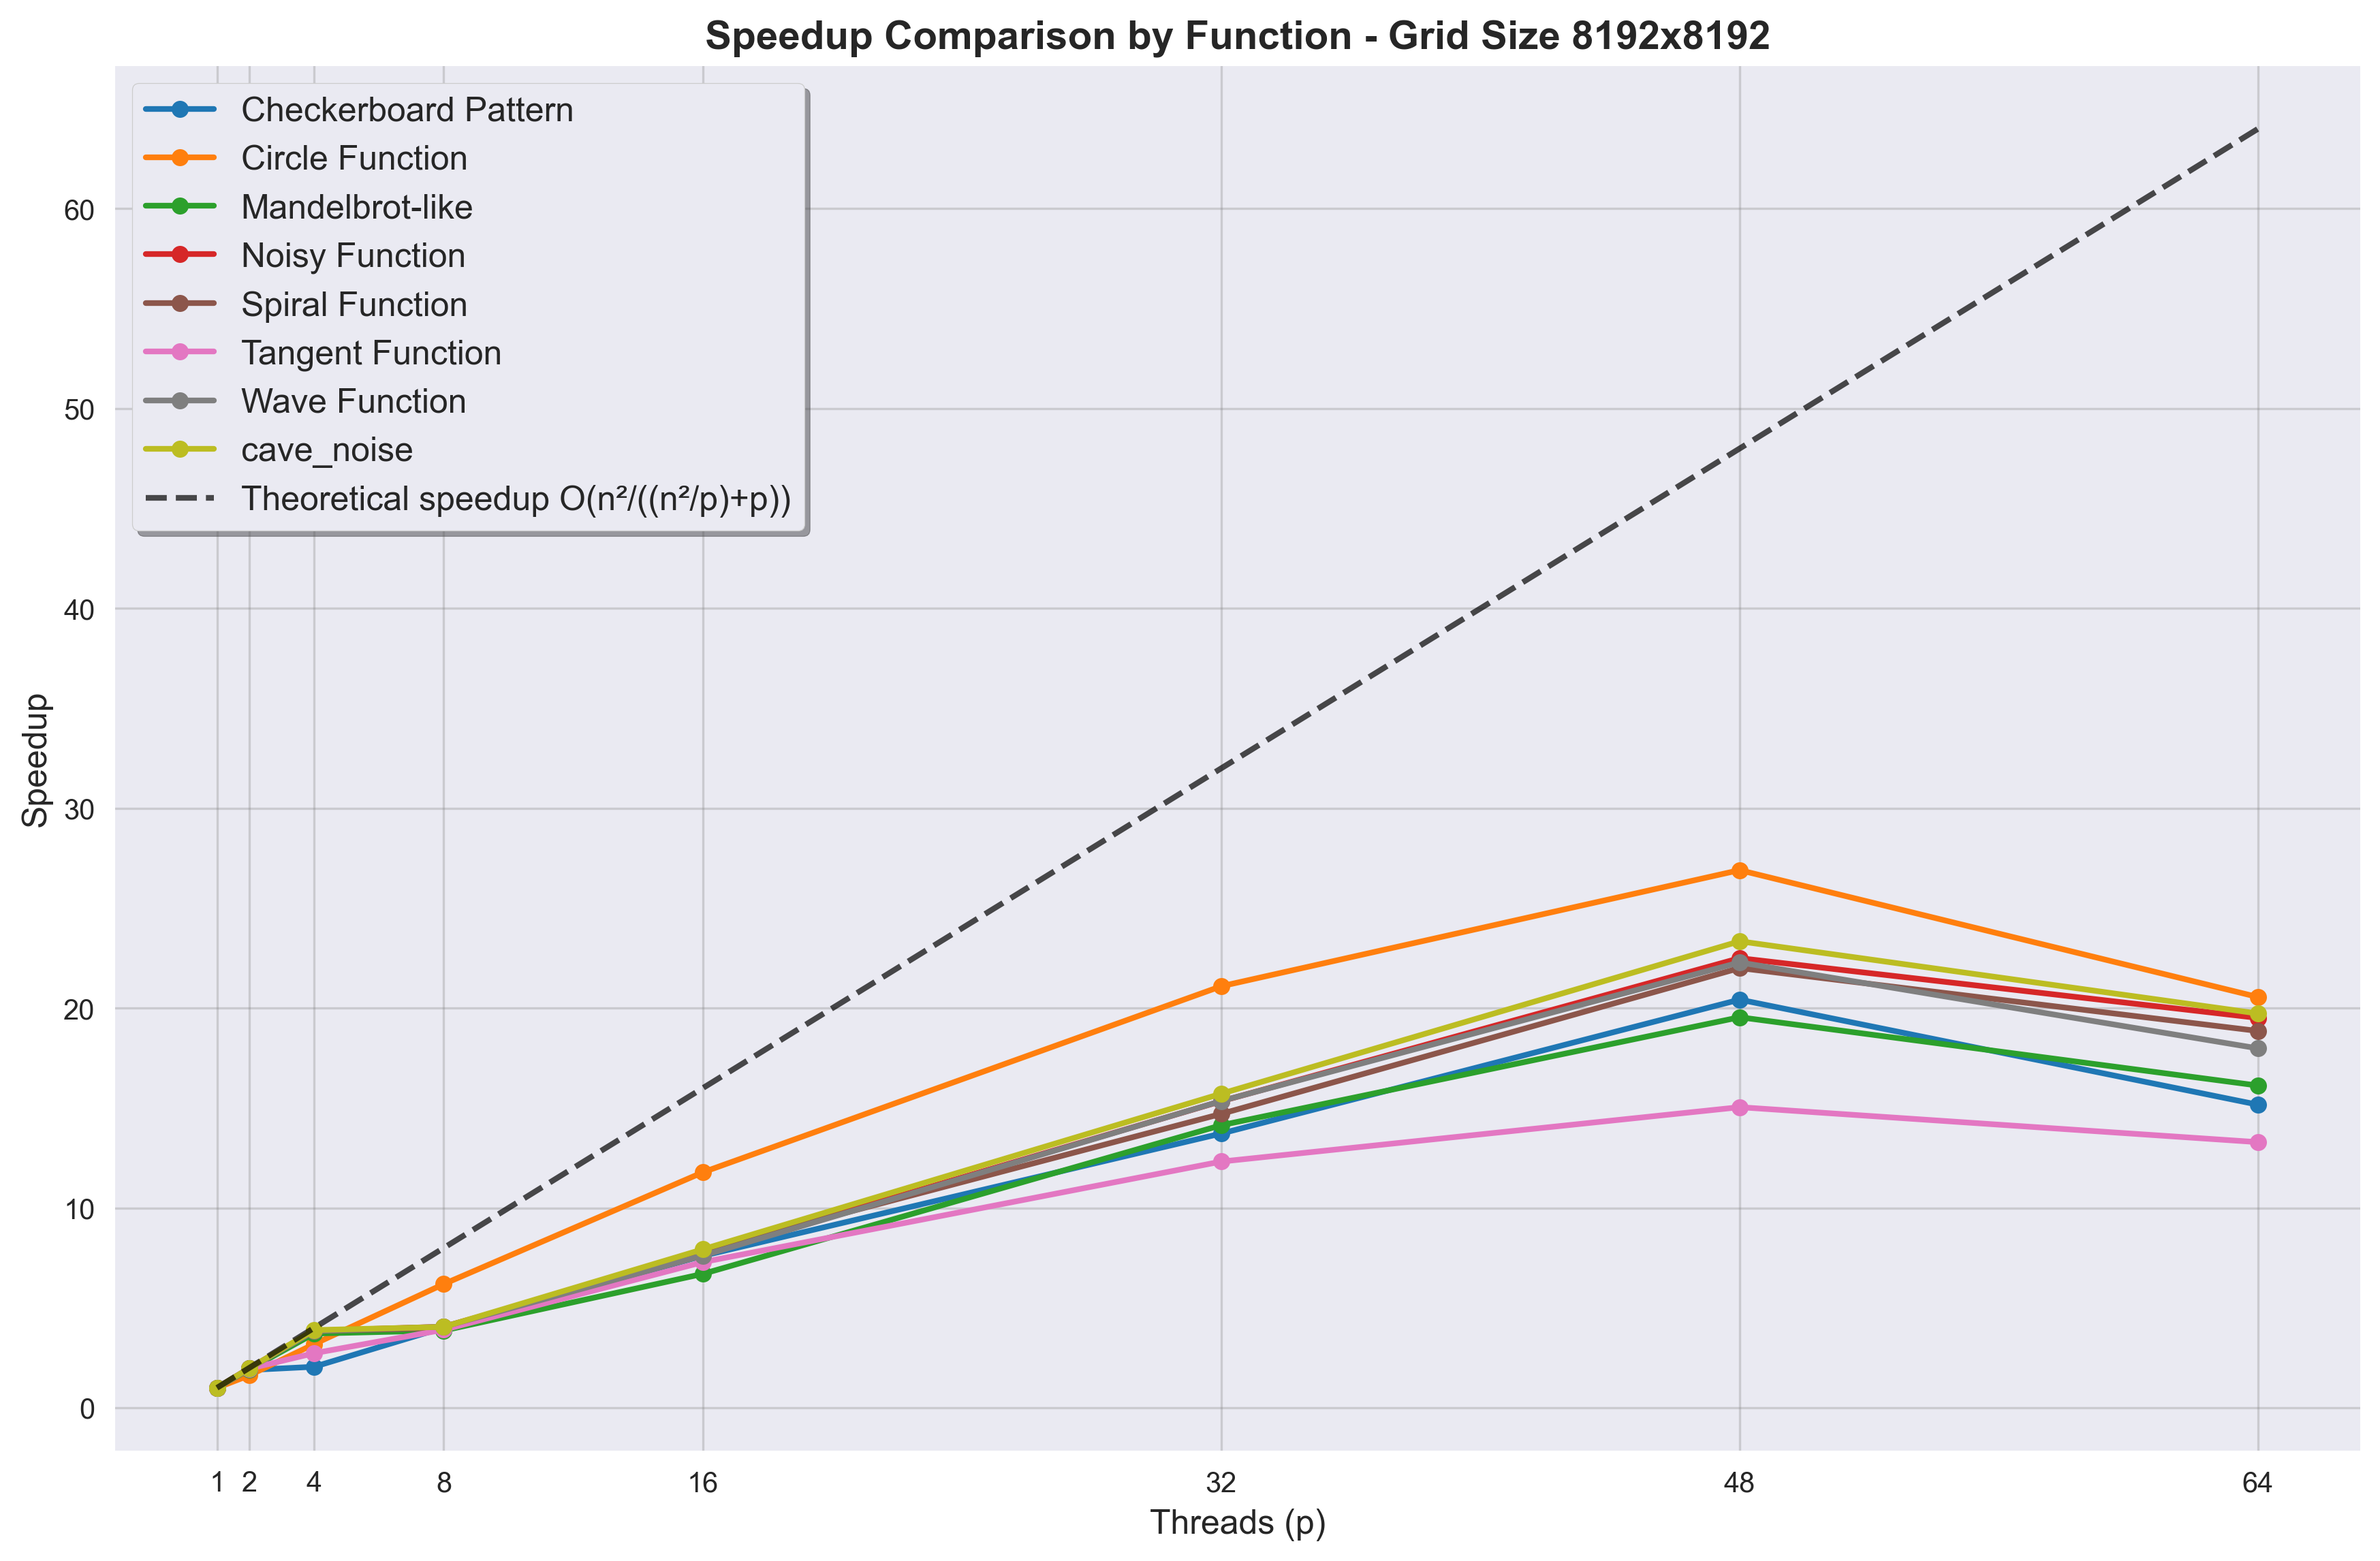
\includegraphics[height=5cm]{images/speedup_comparison_grid_8192.png}
        \caption{Grilla 8192}
        \label{fig:speedup_8192}
    \end{subfigure}\hspace*{\fill}
    \begin{subfigure}{0.48\textwidth}
        \centering
        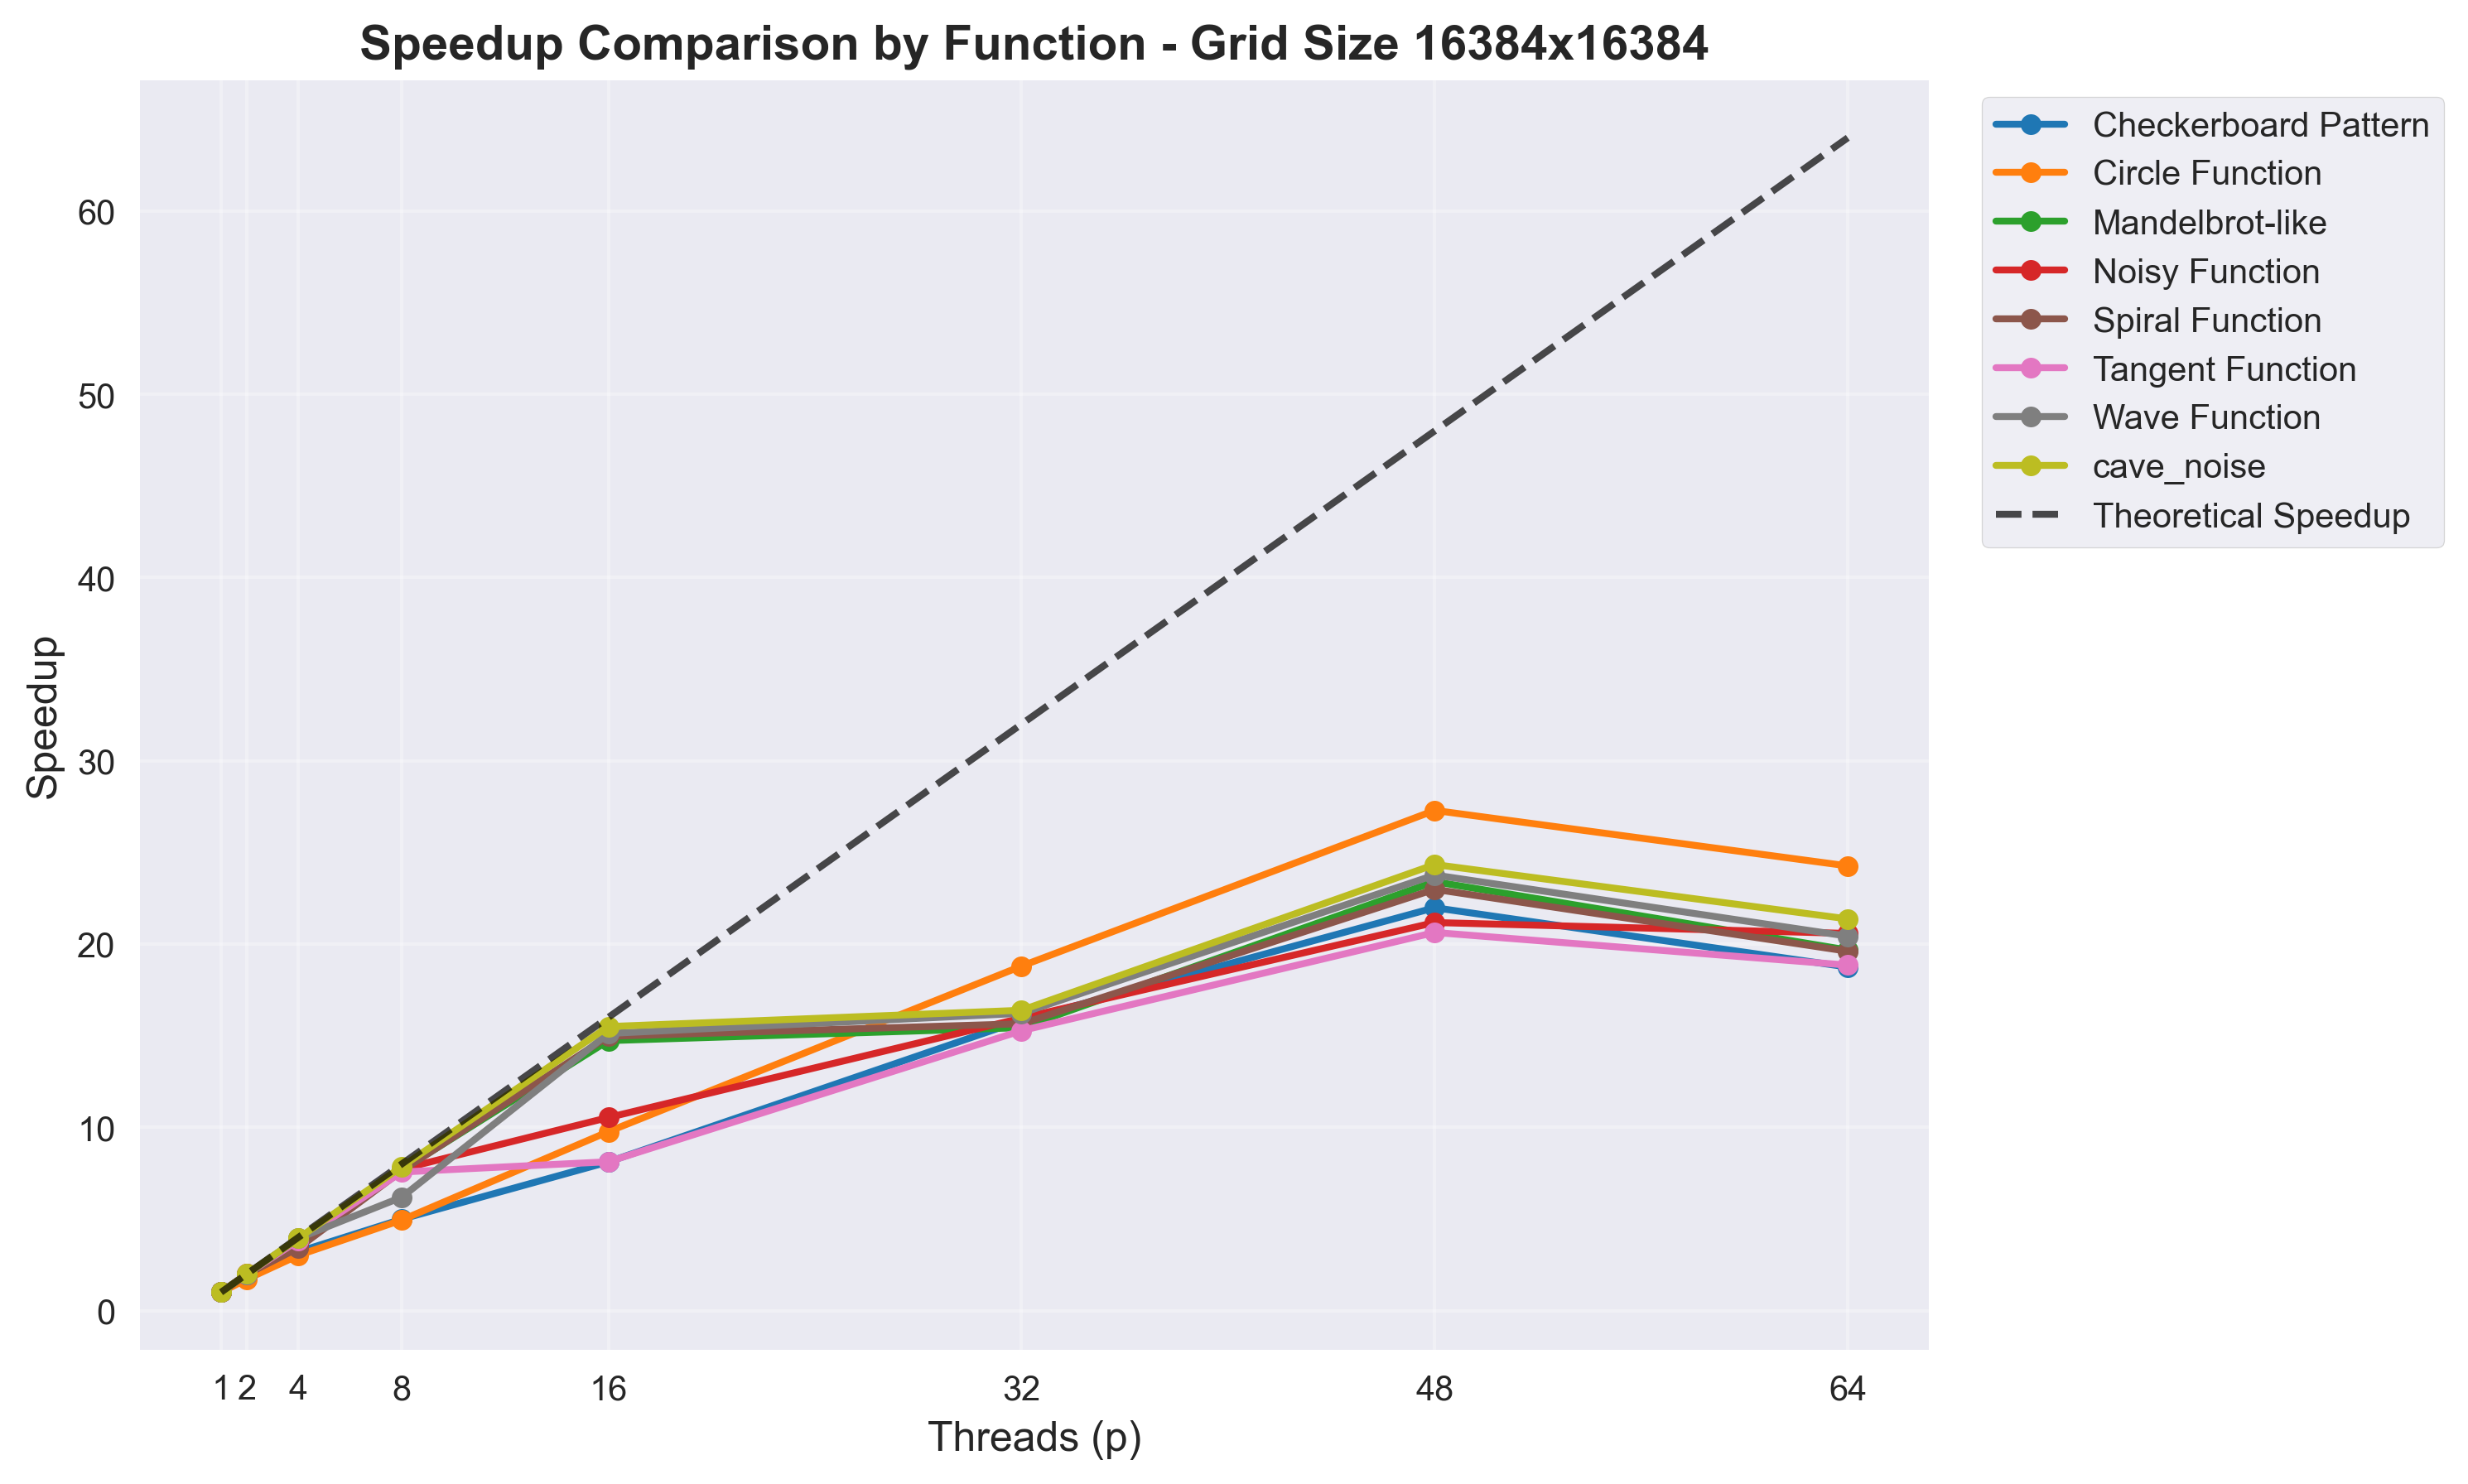
\includegraphics[height=5cm]{images/speedup_comparison_grid_16384.png}
        \caption{Grilla 16384}
        \label{fig:speedup_16384}
    \end{subfigure}

    \caption{Speedup para diferentes tamaños de grilla}
\end{figure}

Los resultados muestran escalabilidad efectiva hasta aproximadamente 32 cores, con eficiencias superiores al 80\% para grillas grandes. La implementación optimizada (Iteración III) alcanza speedups de hasta 130x en configuraciones favorables.

\section{Conclusiones}

La evolución de implementaciones demuestra mejoras progresivas: de 47\% (It2) a 85\% (It3) hasta 95\%+ (It4) en eficiencia paralela. Las optimizaciones clave incluyen \textit{move semantics}, indexación directa por thread y paralelismo masivo en GPU.

El uso de aritmética de doble precisión garantiza exactitud numérica, mientras que la ejecución en Khipu con SLURM permite escalamiento eficiente en entornos de alto rendimiento.

\section{Referencias}
\begin{enumerate}
    \item OpenMP Architecture Review Board. \textit{OpenMP Application Programming Interface Version 5.0}. 2018.
    \item NVIDIA Corporation. \textit{CUDA C++ Programming Guide}. 2023.
    \item Lorensen, W.E., Cline, H.E. \textit{Marching Cubes: A high resolution 3D surface construction algorithm}. Computer Graphics, 1987.
    \item Chapman, B., Jost, G., Van Der Pas, R. \textit{Using OpenMP: Portable Shared Memory Parallel Programming}. MIT Press, 2007.
\end{enumerate}

\section{Anexos}
\label{sec:anexos}

El código fuente del proyecto, incluyendo la implementación en C++ y CUDA, se encuentra disponible en el siguiente \href{https://github.com/DavidHerencia/Marching-Squares-Parallel}{repositorio de GitHub}. 


\end{document}